\chapter{Common misconceptions about laser interferometer gravitational-wave antennae}

\section{The sensitivity/bandwidth ``tradeoff''}
There is an argument that exists in various places in the literature when considering the response of the Fabry-Perot resonant arm cavities of a gravitational wave antenna. %NL%
The argument goes something like this:
\begin{itemize}
\item When designing an interferometer, one must choose the finesse of the arm cavities.
\item An increase in the finesse leads to an increase of stored power in the arms, which increases the sensitivity to gravitational waves.
\item The finesse also negatively impacts the bandwidth of the arm cavities. An increase in finesse leads to a reduction in sensitivity to gravitational waves at frequencies higher than the cavity bandwidth.
\item Thus there is a tradeoff between senitivity and bandwidth, and one must choose the arm cavity finesse to balance the benefits of each.
\end{itemize}

Noise sources that are frequency independant (white) at the photodetector will have a frequency dependent structure shaped as the inverse of the interferometer optical sensitivity. %NL%
In other words, as the interferometer sensitivity decreases, the contribution from that noise source to limiting the ultimate measurement correspondingly increases. %NL%
So sometimes the above argument is given in terms of the shape of the shot noise contribution (which is white at the photodetector) of the interferometer. %NL%
In that case, the argument might say that an interferometer with a higher finesse will have a lower cavity pole, and hence, the shot noise will begin rising in frequency earlier, ultimately leading to a higher noise floor at high frequencies.

The flaw in the argument arises when one actually compares the effects of the two competing contibutions to the interferometer sensitivity. %NL%
This is well illustrated by considering the shot noise floor of a Michelson Interferometer with Fabry Perot arms (FPMI). %NL%
The amplitude spectral density of shot noise of this interferometer, calibrated as refered to the strain measured by the interferometer is \cite{LIGO}
\begin{equation}
\label{eqn:FPMIshotnoise}
h_{\rm{shot}}^{\rm{FPMI}}=\sqrt{\frac{\pi \hbar \lambda}{c P_{\rm{BS}}}}\left(\frac{\sqrt{1+(4 \pi\tau f)^2}}{4 \pi \tau }\right)=h_{\rm{shot}}^{\rm{MI}}\times \frac{\pi\sqrt{1+(4\mathcal{F})^2(f/\rm{FSR})^2}}{2 \mathcal{F}},
\end{equation}
where $\hbar$ is the reduced Planck constant, $\lambda$ is the laser wavelength, $c$ is the speed of light, $P_{\rm{BS}}$ is the light incident on the beam splitter, $\tau=\frac{\mathcal{F}}{\pi \rm{FSR}}$ is the light storage time of the arm cavities, $\rm{FSR}$ is the cavity free spectral range, and $\mathcal{F}$ is the cavity finesse. %NL%
The second equality shows the shot noise scaled by the shot noise in a Michelson interferometer with no cavity arms. %NL%
Equation \ref{eqn:FPMIshotnoise} shows how the behavior of the sensitivity of the interferometer depends on the cavity finesse. %NL%
The low frequency sensitivity is indeed improved with an increased finesse, the shot noise decreses. %NL%
However at high frequencies, where $f \gg \rm{FSR}/4\mathcal{F}$, the effect of the finesse cancels out, and an increase in finesse does not reduce the sensitivity of the interferometer. %NL%
Figure \ref{fig:fpmishotnoise} shows how the shot noise sensitivity changes as a result of changing the arm cavity finesse. %NL%
As one can see, the high frequency sensitivities are all the same. %NL%
So there is no trade-off, an increase in finesse can only benefit the sensitivity, at least in this simplified case.\footnote{This no longer is true, for example, when losses are included.}

\begin{figure}
  \begin{center}
  \leavevmode
  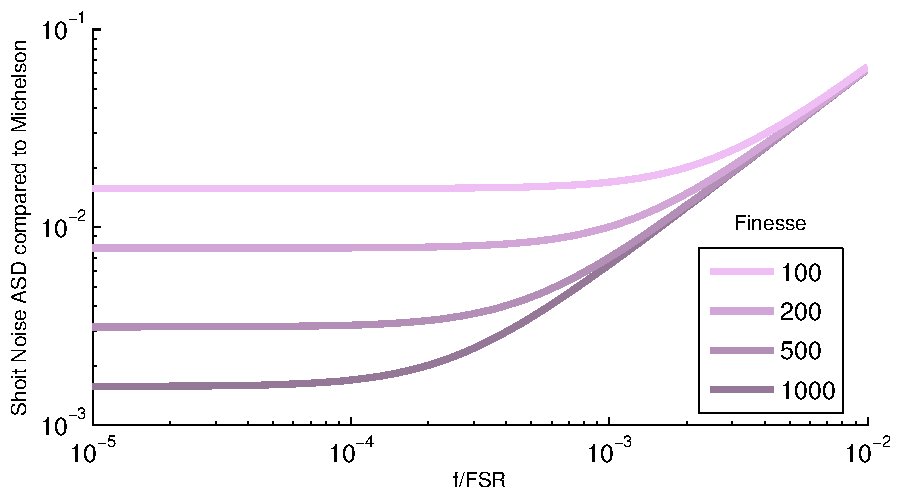
\includegraphics{figs-ap-miscon/fpmishotnoise.pdf}
  \end{center}
  \caption[]{}
  \label{fig:fpmishotnoise}
\end{figure}

In reality, there are good reasons to limit the finesse of the arm cavities. %NL%
These include difficulty of lock acuisition, the ability to deal with very large amounts of stored power in the arm, and the fact that the loss experienced in one round trip through the arm is multiplied by the number of bounces the light experiences.

The choice of the arm cavity finesse for a FPMI is usually driven by the existence of other noise sources. %NL%
The finesse can be increased until other, low frequency, noise sources dominate and there is no benefit to increase the finesse further.

In the case of a FPMI, the finesse governs both the stored arm power and the bandwidth of the differential mode interferometer, or the recycling of the gravitational wave audio sidebands. %NL%
The addition of a signal recycling/extraction mirror, as in Advanced LIGO, breaks this symmetry. %NL%
The signal mirror can be used to modify the detector bandwidth, without changing the stored arm cavity power.

The author is not certain about where this misconception comes from. %NL%
For example, it is treated correctly in the classic reference by \citet{saulson1994fundamentals}. %NL%
On page 103, about the high frequency regime, he writes, ``Further increase in the finesse of the arm cavities neither helps, nor in this simple case hurts, the sensitivity.''

\section{Why LIGO has two arms}
This misconception is alluded to in Section \ref{sec:michelson}, but is treated here more directly. %NL%
People who are knowledgeable about LIGO, but are not familiar with the details of the interferometer are often surprised to learn that the main reasons driving the use of a Michelson interferometer, with two long arms, are related to the coupling of technical noise sources, and not because of the fact that gravitational waves stretch along perpendicular axes.

A Michelson interferometer with symmetric arms bestows the experimentalist with the powerful gift of \emph{common mode noise rejection}. %NL%
Technical fluctuations of the laser amplitude and frequency tend to reflect back to the laser, not to the dark fringe of the Michelson. %NL%
The added benefit of the common mode servo (Section \ref{sec:armcav}) also can be used to reduce the laser frequency noise. %NL%
Again, this is treated beautifully in Sections 10.1.4 and 12.6 of \citet{saulson1994fundamentals}. %NL%


A two-armed interferometer is a significant increase in complexity, though the signal strength is only two times that of a one-armed interferometer. %NL%
It is the massive reduction of noise that makes the complexity worthwile.

\section{With a DARM offset, is LIGO still a null measurement?}
This is not a misconception {\it per se}, but is an intersting point that deserves a small bit of discussion.
